\documentclass{article}
\usepackage{minted}
\usepackage{graphicx} % Required for inserting images
\usepackage{amsmath,amssymb}
\usepackage[letterpaper,top=2cm,bottom=2cm,left=2cm,right=2cm,marginparwidth=1.75cm]{geometry}
\usepackage{color}
\usepackage{braket}
\usepackage{float}
\usepackage{tikz}
\usetikzlibrary{quantikz2}
\usepackage{hyperref}
%\usepackage{comment}
\hypersetup{
    colorlinks = true,
    linkcolor = blue,
    urlcolor = magenta,
    citecolor = magenta
}

\title{Introduction to Quantum Programming}
\author{Ugo Nzongani}
\date{\vskip 0.5cm}

\begin{document}

%\newcommand{\ex}{\textbf{Question. }}

\maketitle

\tableofcontents

\vskip 1cm

\begin{figure}[H]
    \centering
    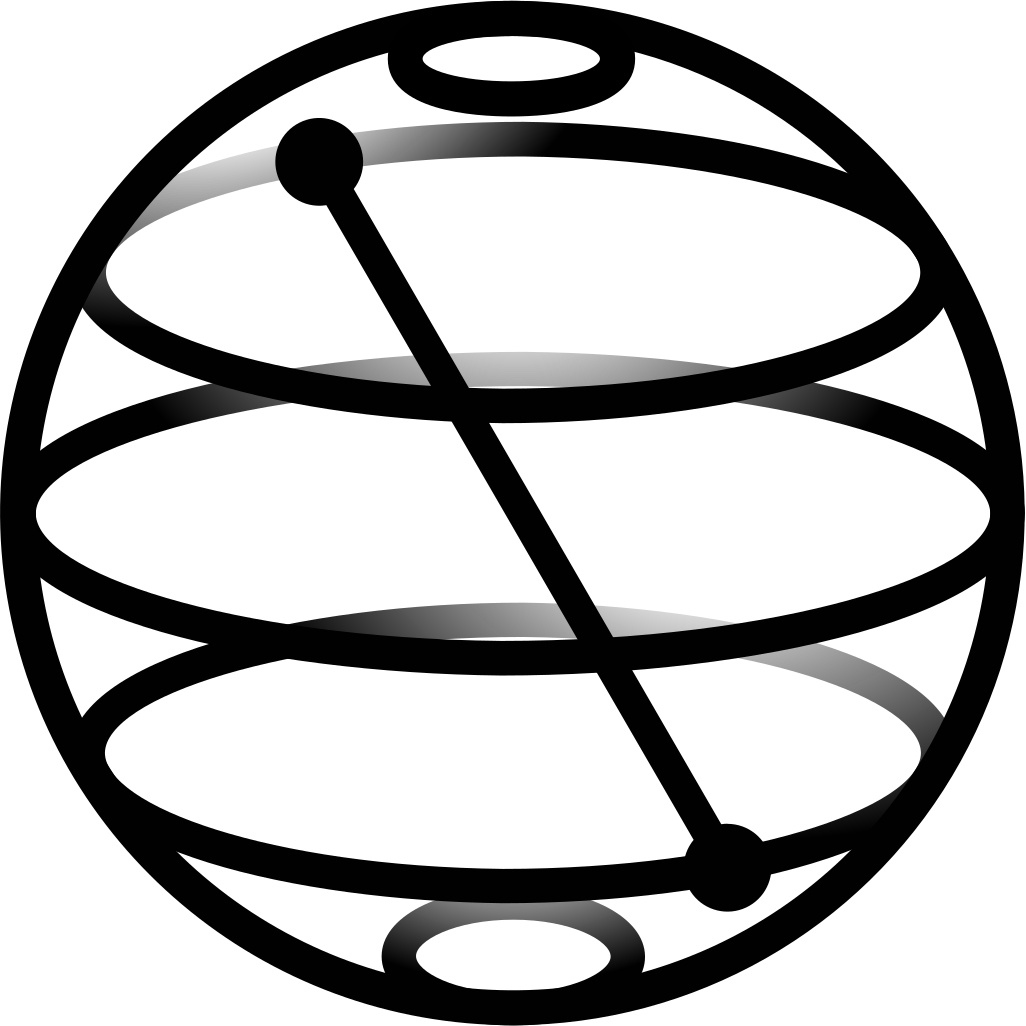
\includegraphics[scale=0.13]{qiskit.png}
\end{figure}

\newpage

\section{Introduction}

\subsection{Libraries}

Quantum programming can be done using several programming libraries, we are going to use \href{https://qiskit.org/}{Qiskit} which is a Python library for quantum computing \cite{qiskit2024}. With Qiskit we can run our code on IBM real quantum devices. It is strongly advised to install a specific virtual environment. Here are the steps to do it:
\begin{minted}{shell-session}
python3 -m venv my_env
source my_env/bin/activate
\end{minted}
Then run the following commands:
\begin{minted}{shell-session}
pip install jupyter
pip install wheel
pip install ipykernel
pip install pylatexenc
\end{minted}

All the necessary libraries are in \verb|requirements.txt|, to install them run \verb|pip install -r requirements.txt|. The imports and functions are in \verb|utils.py|, they can be imported in your file with the line \verb|from utils import *|. One can leave the virtual environment with the command \verb|deactivate|.

\subsection{Introduction to Qiskit}

\subsubsection{Quantum circuit}

A circuit in Qiskit in composed of quantum and classical registers. The quantum registers are used to perform the quantum computations, and the classical ones to store the classical outcome of the measurements. In Qiskit a register is always initialize in state $\ket{0}$.

\begin{minted}{python}
n = 3
m = n
# Quantum register of n qubits
q = QuantumRegister(n, name='q')
# Classical register of m bits
c = ClassicalRegister(m, name='c')
# Quantum circuit
qc = QuantumCircuit(q,c)
# Apply X on qubit 0
qc.x(q[0])
# Apply H on qubit 0
qc.h(q[0])
# Apply a CNOT on qubit 0 controlled by qubit 2
qc.cx(q[2],q[0])
# Put a barrier between the operations
qc.barrier()
# Measure of the register q, the results are stored in c
qc.measure(q,c)
# Drawing the circuit
qc.draw('mpl')
# Note that the display style of the circuit can be modified with:
# qc.draw('mpl',style'bw'), qc.draw('mpl',style'iqx') or qc.draw()
\end{minted}
Once a quantum circuit is created, one can run it to get some outcomes.

\begin{minted}{python}
simulator = AerSimulator()
result = simulator.run(transpile(qc, simulator),shots=1024).result()
counts = result.get_counts()

# Plot the results of the measurements
plot_histogram(counts)
\end{minted}
The variable \verb|counts| is a dictionary that contains the results of the measurements. The keys are the bit string measured and the values corresponds to the number of times this string has been measured. Hence, the dictionary \verb|{'00':134,'01':237,'10':511,'11':118}| indicates that we measured the state $\ket{00}$ 134 times, $\ket{01}$ 237 times, $\ket{10}$ 511 times and $\ket{11}$ 118 times. \\\\ It is also possible to only measure some qubits of the system:

\begin{minted}{python}
# Measure of the qubit 0 of the register q
qc.measure(q[0],c[0])
\end{minted}
The top wire corresponds to the qubit encoding the least significant bit. Let $\ket{x_2x_1x_0}=\ket{000}$ be a quantum state, we want to apply a NOT gate on $\ket{x_0}$, its Qiskit circuit is:
\begin{figure}[H]
    \centering
    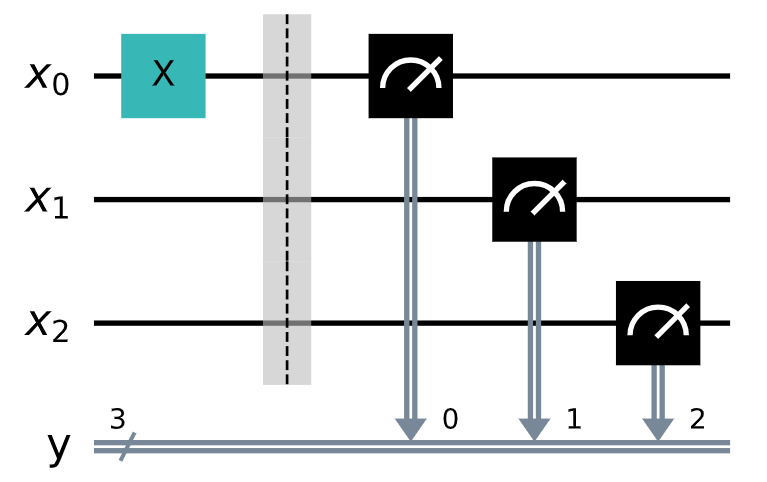
\includegraphics[scale=0.4]{circ1.png}
\end{figure}
The outcome of the measurement is 001 with probability 1.

\subsubsection{Sub-circuit}

It is possible to transform a quantum circuit into a unitary gate, one can see it as a subroutine. Let's create a simple circuit:

\begin{minted}{python}
q = QuantumRegister(2,name='q')
qc = QuantumCircuit(q)
qc.cx(q[0],q[1])
qc.h(q)
\end{minted}
We transform it into a unitary gate:
\begin{minted}{python}
gate = qc.to_gate(label='gate')
\end{minted}
We can now add it as a subroutine in other quantum circuits:
\begin{minted}{python}
q = QuantumRegister(4,name='q')
qc = QuantumCircuit(q)
qc.x(q)
# We apply the gate on the qubits 1 and 2 of the new circuit
qc.append(gate,[q[1],q[2]])
# We apply the same gate on the qubits 1 and 2 of the new circuit but controlled by qubit 0
qc.append(gate.control(),[q[0],q[1],q[2]])
qc.draw('mpl')
\end{minted}
Then, we can decompose the boxes we just created:
\begin{minted}{python}
qc.decompose().draw('mpl')
\end{minted}
To increase the level of the decomposition, the parameter \verb|reps| can be used:
\begin{minted}{python}
qc.decompose(reps=1).draw('mpl')
\end{minted}
We can compute the inverse, power or control gate easily:
\begin{minted}{python}
q = QuantumRegister(5,name='q')
qc = QuantumCircuit(q)
# We apply the gate^2 on the qubits 1 and 2
qc.append(gate.power(2),[q[1],q[2]])
# We apply the inverse of the gate on the qubits 1 and 2
qc.append(gate.inverse(),[q[1],q[2]])
# We apply the gate on the qubits 2 and 3 controlled by qubits 0 and 1
qc.append(gate.control().control(),[q[0],q[1],q[2],q[3]])
qc.draw('mpl')
\end{minted}
\subsubsection{From unitary to gate}
We can convert a unitary matrix into a quantum gate, let's create the gate $U=\begin{pmatrix}
    1 & 0 \\ 0 & e^{i\pi/7}
\end{pmatrix}$:
\begin{minted}{python}
q = QuantumRegister(2,name='q')
qc = QuantumCircuit(q)
U = np.array([[1,0],[0,np.exp(1j*np.pi/7)]])
op = Operator(U)
qc.unitary(op,[q[0]],label='U')
qc.draw('mpl')
\end{minted}

\subsubsection{Run on IBM quantum device}

To run your code on IBM real quantum computer, you first have to create an account on \href{https://quantum-computing.ibm.com/}{IBM Quantum Experience} to get your API Key. Once it is done, you can run the following code:

\begin{minted}{python}
# Bell quantum circuit
q = QuantumRegister(2, name='q')
c = ClassicalRegister(2, name='c')
qc = QuantumCircuit(q, c, name='Bell')
qc.h(q[0])
qc.cx(q[0], q[1])
qc.measure(q, c)

# Running it on IBM real device #

token = 'your_token'

# Show the available IBM devices
devices(token)

# Run the circuit on the specified device, if no device is given the circuit is run on the least busy one
counts = run_ibm(qc,token,device=None)
print(counts)
\end{minted}

\subsection{Usefull functions}

One is encouraged to use the following functions defined in \verb|utils.py| to run its circuit on a simulator and to plot quantum states:
\begin{itemize}
    \item You can run a quantum circuit on a simulator with \verb|run(qc,n_shots=1024,plot=True)|, the parameters \verb|n_shots| and \verb|plot| are optional. The first indicates the number of execution of the circuit\footnote{As the measure operation is probabilistic one has to execute a circuit several times to obtain a reliable probability distribution.}, if the second is set to \verb|False| the function returns a dictionnary containing the results of the execution.
    \item You can plot a quantum state with \verb|draw_state(qc,latex=False)|, the parameter \verb|latex| is optional and if set to \verb|True| the function displays the mathematical expression of the quantum state, otherwise the outcome is the Bloch Sphere of the state.
\end{itemize}


\newpage

\section{First quantum circuits}

\begin{enumerate}
    \item Plot the Bloch Sphere representation of the states $\ket{0}$,$\ket{1}$, $\frac{1}{\sqrt{2}}(\ket{0}+\ket{1})$ and $\frac{1}{\sqrt{2}}(\ket{0}-\ket{1})$. Here is the code for $\ket{0}$:
    \begin{minted}{python}
    q = QuantumRegister(1)
    qc = QuantumCircuit(q)
    bloch(qc,latex=False)
    \end{minted}
    If \verb|latex| is set to \verb|False| the output is the Bloch Sphere representation of the qubit state, otherwise it is the mathematical expression.
    \item Do the same with the state $\ket{\psi}=\frac{1}{\sqrt{2}}(\ket{00}+\ket{01})$. 
    \item Lastly, do it for the state $\ket{\Psi}=\frac{1}{\sqrt{2}}(\ket{00}+\ket{11})$. Can you explain what is happening ?
    \item Design a quantum circuit that creates the state $\ket{\psi}=\frac{1}{2}(\ket{00}+\ket{01}+\ket{10}+\ket{11})$, run it and plot the measurement results, or display its statevector.
    \item Design a quantum circuit that creates the state $\ket{\psi}=\frac{1}{\sqrt{2}}(\ket{000}+\ket{111})$, run it and plot the measurement results, or display its statevector.
     \item Design a quantum circuit that creates the state $\ket{\psi}=\frac{i}{\sqrt{2}}(\ket{010}-\ket{110})$\footnote{\textit{Hint: you only have to use $X,Y$ and $H$ gates.}} and display its statevector. Note that its Bloch Sphere representation is:
     \begin{figure}[H]
         \centering
         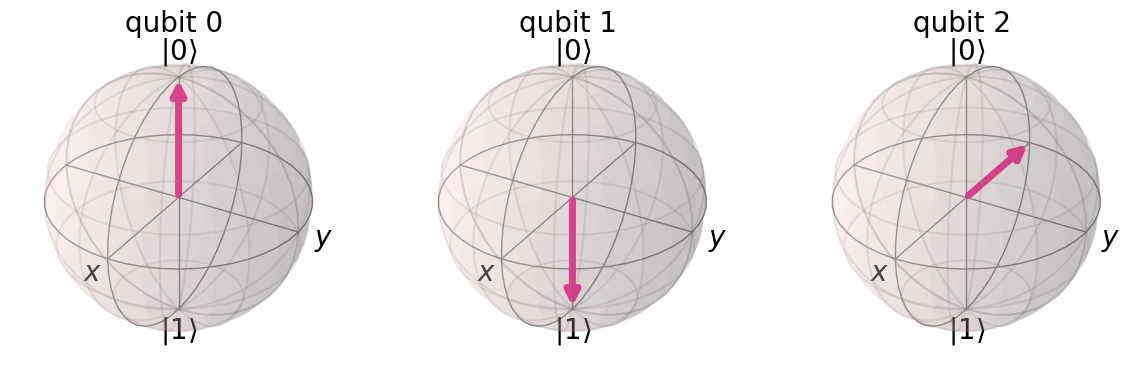
\includegraphics[scale=0.35]{bloch3.png}
     \end{figure}
    \item Using the function \verb|random_unitary|, create a random state $\ket{\psi}$. Design a quantum circuit working on the state $\ket{\psi}\otimes\ket{0}$ that swaps these two qubits into:
    \begin{equation*}
        \ket{\psi}\otimes\ket{0} \mapsto \ket{0}\otimes\ket{\psi}
    \end{equation*}
    Plot its Bloch Sphere representation before and after to check the result of the computation.
    \item One wishes to design a quantum circuit that performs the following transformation on $n$ qubits:
    \begin{equation*}
        \sum_{k=0}^{2^n-1}\alpha_k\ket{k} \mapsto \sum_{k=0}^{2^n-1}\alpha_k\ket{2^n-1-k}
    \end{equation*}
    Note that it should work for any $(\alpha_0,\dots,\alpha_{2^n-1})\in \mathbb{C}^{2^n}$, not only for $\alpha_k=\frac{1}{\sqrt{2^n}}$. This transformation is just a permutation of the amplitudes $\alpha_k$ over the basis states, creating some kind of “mirror quantum state”. Let's take an example with $n=2$ qubits, in such a case this mapping acts as:
    \begin{equation*}
        \begin{split}
            \alpha_0\ket{00} &\mapsto \alpha_0\ket{11} \\
            \alpha_1\ket{01} &\mapsto \alpha_1\ket{10} \\
            \alpha_2\ket{10} &\mapsto \alpha_2\ket{01} \\
            \alpha_3\ket{11} &\mapsto \alpha_3\ket{00}
        \end{split}
    \end{equation*}
    \begin{enumerate}
        \item Make a list \verb|unitaries| of length $n$ that contains random $2\times 2$ unitaries.
        \item Design a quantum circuit \verb|qc1| that creates the state $\sum_{k=0}^{2^n-1}\alpha_k\ket{k}$, where the $\alpha_k$ are that of \verb|unitaries|.
        \item Design a quantum circuit \verb|qc2| that creates the state $\sum_{k=0}^{2^n-1}\alpha_k\ket{2^n-1-k}$, where the $\alpha_k$ are that of \verb|unitaries|.
        \item Run the quantum circuits and plot their results, both plots should mirror one another.\\ It is possible to plot results from 2 quantum circuit at once with:\\ \verb|plot_histogram([run(qc1, plot=False),run(qc2, plot=False)])|
    \end{enumerate}
    \item Reproduce the following quantum circuit, try to do it using as little code as possible:
    \begin{figure}[H]
    \centering
    \scalebox{0.7}{
    \begin{quantikz}
    \lstick{$\ket{0}$} & \octrl{3} & \gate{P(\pi)} & \ctrl{3} & \gate{P(2\pi)} & \octrl{3} & \gate{P(3\pi)} & \ctrl{3} & \gate{P(4\pi)} & \octrl{3} & \gate{P(5\pi)} & \ctrl{3} & \gate{P(6\pi)} & \octrl{3} & \gate{P(7\pi)} & \ctrl{3} & \gate{P(8\pi)} & \qw \\
    \lstick{$\ket{0}$} & \octrl{2} & \gate{P(\pi/2)} & \octrl{2} & \gate{P(\pi)} & \ctrl{2} & \gate{P(3\pi/2)} & \ctrl{2} & \gate{P(2\pi)} & \octrl{2} & \gate{P(5\pi/2)} & \octrl{2} & \gate{P(3\pi)} & \ctrl{2} & \gate{P(7\pi/2)} & \ctrl{2} & \gate{P(4\pi)} & \qw \\
    \lstick{$\ket{0}$} & \octrl{1} & \gate{P(\pi/4)} & \octrl{1} & \gate{P(\pi/2)} & \octrl{1} & \gate{P(3\pi/4)} & \octrl{1} & \gate{P(\pi)} & \ctrl{1} & \gate{P(5\pi/4)} & \ctrl{1} & \gate{P(3\pi/2)} & \ctrl{1} & \gate{P(7\pi/4)} & \ctrl{1} & \gate{P(2\pi)} & \qw \\
    \lstick{$\ket{1}$} & \targ{} & \gate{H} & \targ{} & \gate{H} & \targ{} & \gate{H} & \targ{} & \gate{H} & \targ{} & \gate{H} & \targ{} & \gate{H} & \targ{} & \gate{H} & \targ{} & \gate{H} & \qw
\end{quantikz}}
\end{figure}
The phase gate $P(\theta)=\begin{pmatrix}
    1 & 0 \\ 0 & e^{i\theta}
\end{pmatrix}$ can be used with \verb|qc.p(theta,qubit)|, the multi-controlled NOT-gate can be used with \verb|qc.mcx|, one is encouraged to check its documentation \href{https://docs.quantum.ibm.com/api/qiskit/qiskit.circuit.library.MCXGate}{here}. Lastly, one should remember the identity:
\begin{figure}[H]
    \centering
    \begin{quantikz}
    \qw & \octrl{1} & \qw \\
    \qw & \targ{} & \qw
\end{quantikz}
=
\begin{quantikz}
    \qw & \targ{} & \ctrl{1} & \targ{} & \qw \\
    \qw & \qw & \targ{} & \qw & \qw
\end{quantikz}
\end{figure}
\item Can you generalize the previous circuit for $n>1$ qubits knowing that it was $n=3$?
\end{enumerate}

\section{Cloning qubits ?}
In quantum computing it is not possible to copy an arbitrary qubit state $\alpha\ket{0}+\beta\ket{1}$ due to the No-Cloning theorem. Hence, such a transformation is impossible for arbitrary $\ket{\psi}$:
\begin{equation*}
    \ket{\psi}\ket{0} \mapsto \ket{\psi}\ket{\psi}
\end{equation*}
However, it does not mean that any kind of copy is impossible, let's try some experiments. Unknown quantum states can be prepared using the function \verb|random_unitary|.

\begin{enumerate}
    \item Given a quantum state $\ket{a}=\ket{0}$ or $\ket{a}=\ket{1}$, design a quantum circuit that performs the following computation:
    \begin{equation*}
        \ket{a}\otimes\ket{0} \mapsto \ket{a}\otimes\ket{a}
    \end{equation*}
    \item Can you still find a circuit to do it when the second qubit is initialized to $\ket{1}$ ?
    \begin{equation*}
        \ket{a}\otimes\ket{1} \mapsto \ket{a}\otimes\ket{a}
    \end{equation*}
     \item Given a quantum state $\ket{a=a_n\dots a_1}=\ket{a_n}\otimes\cdots\otimes\ket{a_1}$ with $a_i\in \{0,1\}$, design a quantum circuit that performs the following computation:
    \begin{equation*}
        \ket{a_n\dots a_1}\otimes\ket{0}^{\otimes n} \mapsto \ket{a_n\dots a_1}\otimes\ket{a_n\dots a_1}
    \end{equation*}
    \item In questions (1) and (2), we made quantum circuits that copy the bit value of a qubit into an ancilla qubit. We now wish to do the same operation for $n$ ancilla qubits, that is:
    \begin{equation*}
        \ket{a}\otimes\ket{0}^{\otimes n} \mapsto \ket{a}\otimes \ket{a}^{\otimes n}
    \end{equation*}
    \begin{enumerate}
        \item Design a quantum circuit that performs this operation for $n\in \mathbb{N}^*$.
        \item The quantum circuit you just made probably has a time complexity of $O(n)$, i.e. a linear scaling with the number of ancilla qubits. Can you improve it to obtain a logarithmic scaling, i.e. $O(\log_2 n)$?
        \item Plot the quantum circuit execution time evolution as a function of the number of ancilla qubits, for the linear and logarithmic methods. The time execution can be obtained with \verb|qc.depth()|.
    \end{enumerate}
    
\end{enumerate}

\section{Single qubit interference}

Interferences play a major role in quantum computation, by going into the Fourier basis (applying a Hadamard on a single qubit) and applying a phase it is possible to create an interesting interference scheme as depending on the value of the phase, the outcome of the measurement will change.

\begin{figure}[H]
    \centering
    \begin{quantikz}
        \lstick{$\ket{0}$} & \gate{H} & \phase{\varphi} & \gate{H} & \qw
    \end{quantikz}
\end{figure}

\begin{enumerate}
    \item Implement the single qubit interference circuit with the phase gate $P(\varphi) = \begin{pmatrix}
        1 & 0 \\ 0 & e^{i\varphi}
    \end{pmatrix}$.
    \item Plot the probabilities of measuring $\ket{0}$ and $\ket{1}$ as a function of $\varphi$, you can access the statevector \verb|psi| of the circuit by adding the following lines at the end:
    \begin{minted}{python}
            qc.save_statevector()
            simulator = AerSimulator()
            psi = simulator.run(qc).result().get_statevector(qc)
    \end{minted}
\end{enumerate}

\section{Superdense coding}

The Superdense coding protocol \cite{bennett1992communication} corresponds to the following quantum circuit:

\begin{figure}[H]
    \centering
    \begin{quantikz}
    \lstick{$\ket{0}_A$} & \gate{H} & \ctrl{1} & \gate{U} & \ctrl{1} & \gate{H} & \meter{} & \cw & \rstick{$b_1$}\qw \\
    \lstick{$\ket{0}_B$} & \qw & \targ{} & \qw & \targ{} & \qw & \meter{} & \cw & \rstick{$b_2$}\qw
\end{quantikz}
\end{figure}

Note that the black box $U$ corresponds to the operations performed by Alice depending on the informations she wants to send. Write a function \verb|Superdense_Coding(b2,b1)| that takes the bits of information Alice wants to send to Bob as inputs, and implements the corresponding Superdense coding protocol.

\section{Quantum Teleportation}

The Quantum Teleportation protocol \cite{bennett1993teleporting} is described with the quantum circuit:

\begin{figure}[H]
    \centering
    \begin{quantikz}[classical gap=0.05cm]
    \lstick{$\ket{\psi}$} & \qw & \qw & \ctrl{1} & \gate{H} & \qw & \meter{} & \cw \\
    \lstick{$\ket{0}_A$} & \gate{H} & \ctrl{1} & \targ{} & \qw & \meter{} & \cw\wire[u]{c} & \cw \\
    \lstick{$\ket{0}_B$} & \qw & \targ{} & \qw & \qw & \targ{}\wire[u]{c} & \gate{Z}\wire[u]{c} & \rstick{$\ket{\psi}$}\qw
    \end{quantikz}
\end{figure}
    
\begin{enumerate}
    \item Implement the Quantum Teleporation protocol.
    \item Plot the Bloch Sphere of the 3 qubits system before and after teleportation. Do not forget to generate a random quantum state for the state $\ket{\psi}$ to teleport. Note that the state before teleportation is $\ket{\psi}\otimes \frac{1}{\sqrt{2}}(\ket{0_A0_B}+\ket{1_A1_B})$.
\end{enumerate}

\section{Enumeration}

\begin{enumerate}
    \item Write a function \verb|counting(n)| that takes a number $n$ of qubits as input and returns a quantum circuit that flip sequentially the qubits to generate the following integers:
    \begin{equation*}
        \ket{0} \rightarrow \ket{1} \rightarrow \ket{2} \rightarrow \dots \rightarrow \ket{2^n-1}
    \end{equation*}
    Note that the notation $\ket{2}$ corresponds to the state $\ket{10}$ if working with 2 qubits, it would have been $\ket{010}$ for 3 qubits, etc... Use the line \verb|qc.save_statevector(label=str(i))| to save the statevector of the qubits at iteration $i$. You can nicely visualize the different states of your circuit by running the code:
    \begin{minted}{python}
        simulator = AerSimulator()
        result = simulator.run(qc).result()
        for i in range(2**n):
            psi = result.data(0)[str(i)]
            clear_output(wait=True)
            print('Bloch Sphere representation of '+str(i)+' in the computational basis:')
            display(psi.draw('latex'))
            display(plot_bloch_multivector(psi))
            time.sleep(3)
        clear_output(wait=True)
    \end{minted}
    You can uncomment the line \verb|display(psi.draw('latex'))| to display the mathematical expression instead of the Bloch Sphere of the state. Here is the circuit you should get for $n=3$:
    \begin{figure}[H]
        \centering
        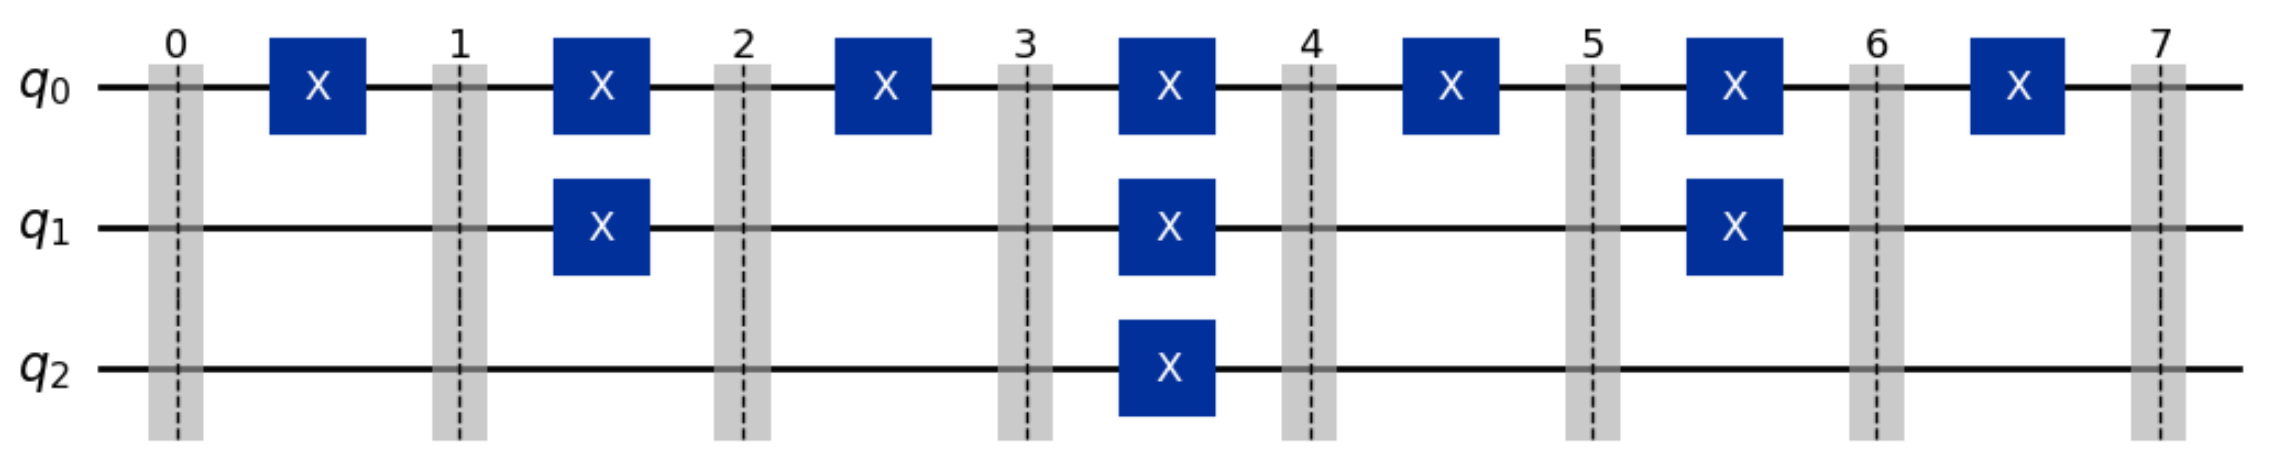
\includegraphics[scale=0.2]{counting.png}
    \end{figure}
    \item The previous circuit is not using the optimal number of $X$ gates because we generated the integers in increasing order. The optimal way of counting is to use Gray code. It is a binary representation of integers where two successive values differ in only one bit. Using this property, one is able to minimize the number of $X$ gates. We show on Fig. \ref{fig:gray} the 3-bits Gray code.
    \begin{figure}[H]
    \centering
    \begin{tabular}{|c|c|c|}
    \hline
    \textit{Decimal with Gray code ordering} & \textit{Binary representation} \\
    \hline
    0 & 000 \\
    \hline
    1 & 001 \\
    \hline
    3 & 011 \\
    \hline
    2 & 010 \\
    \hline
    6 & 110 \\
    \hline
    7 & 111 \\
    \hline
    5 & 101 \\
    \hline
    4 & 100 \\
    \hline
    \end{tabular}
    \caption{3-bits Gray code.}
    \label{fig:gray}
    \end{figure}
    Write a function \verb|gray_counting(n,gray_list)| that takes a number $n$ of qubits, a list of Gray code bitstring of size $2^n$, and returns a quantum circuit that generate the integers from $0$ to $2^n-1$ in Gray code order. Note that for $n=3$ qubits, \verb|gray_list| is: \verb|['000', '001', '011', '010', '110', '111', '101', '100']|.
    \item Plot the number of $X$ gates as a function of the number of qubit $n$ for \verb|counting| and \verb|gray_counting|.
    \end{enumerate}
    
\section{Quantum Fourier Transform}

The Quantum Fourier Transform (QFT) is the quantum analog of the Fourier Transform, it is used as a subroutine in many quantum algorithms. It acts on a quantum state of $n$ qubits, with $N=2^n$, as:
\begin{equation*}
    \ket{x} = \sum_{k=0}^{N-1}x_k\ket{k}
\end{equation*}
and maps it to
\begin{equation*}
    QFT\ket{x} = \sum_{k=0}^{N-1}y_k\ket{k} \mbox{ with } y_k = \frac{1}{\sqrt{N}}\sum_{j=0}^{N-1}x_je^{2\pi i\frac{jk}{N}}
\end{equation*}
The QFT is a transform between the computational basis and the Fourier basis. The computational basis encodes information in the $\ket{k}$ states unlike the Fourier basis that does it in the phases. For more informations, one is encouraged to click \href{https://learn.qiskit.org/course/ch-algorithms/quantum-fourier-transform}{here}.

The quantum circuit implementing the QFT is shown bellow with $R_k=\begin{pmatrix}
    1 & 0 \\ 0 & e^{2\pi i/2^k}
\end{pmatrix}$:

\begin{figure}[H]
    \centering
    \scalebox{0.7}{
    \begin{quantikz}
        \lstick{$\ket{x_{n}}$} & \gate{H} & \gate{R_2} & \gate{R_3} & \qw & \cdots & & \gate{R_n} & \qw & \qw & \qw & \qw & \qw & \qw & \qw & \cdots & & \qw & \qw & \qw & \swap{5} & \qw & \rstick{$\frac{1}{\sqrt{2}}(\ket{0}+e^{2\pi i[0.x_{n}\dots x_1]}\ket{1})$}\qw \\
        \lstick{$\ket{x_{n-1}}$} & \qw & \ctrl{-1} & \qw & \qw & \cdots & & \qw & \gate{H} & \gate{R_2} & \qw & \cdots & & \gate{R_{n-1}} & \qw & \cdots & & \qw & \qw & \qw & \qw & \swap{3} & \rstick{$\frac{1}{\sqrt{2}}(\ket{0}+e^{2\pi i[0.x_{n-1}\dots x_1]}\ket{1})$}\qw \\
        \lstick{$\ket{x_{n-2}}$} & \qw & \qw & \ctrl{-2} & \qw & \cdots & & \qw & \qw & \ctrl{-1} & \qw & \cdots & & \qw & \qw & \cdots & & \qw & \qw & \qw & \qw & \qw & \rstick{$\frac{1}{\sqrt{2}}(\ket{0}+e^{2\pi i[0.x_{n-2}\dots x_1]}\ket{1})$}\qw \\
        \vdots \\
        \lstick{$\ket{x_{2}}$} & \qw & \qw & \qw & \qw & \qw & \qw & \qw & \qw & \qw & \qw & \qw & \qw & \qw & \qw & \cdots & & \gate{H} & \gate{R_2} & \qw & \qw & \targX{} & \rstick{$\frac{1}{\sqrt{2}}(\ket{0}+e^{2\pi i[0.x_2x_1]}\ket{1})$}\qw \\
        \lstick{$\ket{x_{1}}$} & \qw & \qw & \qw & \qw & \qw & \qw & \ctrl{-5} & \qw & \qw & \qw & \qw & \qw & \ctrl{-4} & \qw & \cdots & & \qw & \ctrl{-1} & \gate{H} & \targX{} & \qw & \rstick{$\frac{1}{\sqrt{2}}(\ket{0}+e^{2\pi i[0.x_1]}\ket{1})$}\qw 
    \end{quantikz}
    }
\end{figure}

\begin{enumerate}
    \item Write a function \verb|QFT(n,swaps=True)| that takes the number of qubits $n$ and a boolean \verb|swaps| as inputs, which implements the QFT. The boolean \verb|swaps| indicates if one should include the swap step at the end of the circuit. The controlled-rotations can be implemented with \verb|qc.cp(angle,control_qubit,target_qubit)|.%The controlled-rotations can be implemented with \href{https://qiskit.org/documentation/stable/0.19/stubs/qiskit.circuit.library.U1Gate.html}{U1Gate} or by creating the gate with a numpy array.
    \item Run your function to generate the QFT circuit on 1 qubit. Did you expect this result?
    \item In the previous exercice we enumerated integers from $0$ to $2^n-1$ in the computational basis, i.e. by flipping qubits with $X$ gates. It turns out that we can do the same operations in the Fourier space by doing rotations instead of bit flips. Knowing that $H$ is the QFT on 1-qubit, one should remember the identity:
    \begin{equation*}
        X = HZH
    \end{equation*}
    with
    \begin{equation*}
        Z = \begin{pmatrix}
            1 & 0 \\
            0 & -1
        \end{pmatrix}
        = \begin{pmatrix}
            1 & 0 \\
            0 & e^{i\pi}
        \end{pmatrix}
        = P(\theta=\pi)
    \end{equation*}
    More generally, one can go from basis state $\ket{k}$ to $\ket{k+1\mod 2^n}$ using the following protocol:
    \begin{enumerate}
        \item Apply a QFT to go in Fourier basis (with no swaps)
        \item For each qubit $j\in [0,n-1]$ apply a phase gate $P(\theta)$ with $\theta=2\pi/2^{j+1}$
        \item Apply the inverse QFT to go back to the computational basis (with no swaps)
    \end{enumerate}
    Write a function \verb|fourier_counting(n)| that takes a number $n$ of qubits as input and returns a quantum circuit that sequentially counts integers $k\in [0,2^n-1]$ in Fourier space. Do not forget to retrieve the statevector of the state at each iteration $k$ to visualize the modifications of the corresponding Bloch Spheres:
    \begin{minted}{python}
        simulator = AerSimulator()
        qc_transpile = transpile(qc, simulator)
        result = simulator.run(qc_transpile).result()
        for i in range(2**n):
            psi = result.data(0)[str(i)]
            clear_output(wait=True)
            print('Bloch Sphere representation of '+str(i)+' in the Fourier basis:')
            display(psi.draw('latex'))
            display(plot_bloch_multivector(psi))
            time.sleep(3)
        clear_output(wait=True)
    \end{minted}
    \item The complexity of a quantum circuit is usually defined by its number of 1 and 2 qubit gates. The complexity of the classical Fast Fourier Transform (FFT) is $O(N\log N)$ with $N=2^n$. What is the asymptotic complexity of the Quantum Fourier Transform?
\end{enumerate}

\section{Quantum Phase Estimation}

Quantum Phase Estimation (QPE) is a very usefull subroutine for finding the eigenvalues of a unitary $U$. As it is unitary, its eigenvalue are of the form $e^{2i\pi\varphi}$. Using QPE, one can find the phase $\varphi$ as the outcome of the measurements is $\varphi 2^n$ with high probability. We recall that if $\ket{\psi}$ is an eigenvector of $U$, then $U\ket{\psi}=e^{2i\pi\varphi}\ket{\psi}$ for $\varphi\in \mathbb{R}$. It uses two quantum registers, the eigenvector $\ket{\psi}$ (acting on $m$ qubits) and a working register of $n$ qubits initialized to $\ket{0}$. Here is the quantum circuit implementation of QPE:

\begin{figure}[H]
    \centering
    \begin{quantikz}
        \lstick{$\ket{q_n=0}$} & \gate{H} & \qw & \qw & \qw & \cdots & & \ctrl{4} & \qw & \gate[4]{QFT^{\dagger}} & \qw & \meter{} & \cw \\
        \vdots & & \qw & \qw & \qw & \cdots & & \qw & \qw & \qw & \qw & \vdots \\
        \lstick{$\ket{q_2=0}$} & \gate{H} & \qw & \ctrl{2} & \qw & \cdots & & \qw & \qw & \qw & \qw & \meter{} & \cw\\
        \lstick{$\ket{q_1=0}$} & \gate{H} & \ctrl{1} & \qw & \qw & \cdots & & \qw & \qw & & \qw  & \meter{} & \cw \\
        \lstick{$\ket{\psi}$} & \qwbundle{m} & \gate{U^{2^0}} & \gate{U^{2^1}} & \qw & \cdots & & \gate{U^{2^{n-1}}} & \qw & \qw & \qw & \qw & \qw
    \end{quantikz}
\end{figure}

\begin{enumerate}
    \item Implement the QPE circuit with $m=1$ by writing a function \verb|QPE(n,psi,U)| that takes the number of qubits $n$ initialized to $\ket{0}$, \verb|psi| a unitary to initialize the state of the bottom qubit, and a unitary $U$ as inputs.
    \item To check if your implementation is correct, we are going to estimate the value of $\pi$ using QPE. Let $\ket{\psi}$ be an eigenvector of $U$, therefore $U\ket{\psi}=e^{2i\pi\varphi}\ket{\psi}$. Using QPE we can easily get $\varphi$ since $\varphi=\frac{\delta}{2^n}$, where $\delta$ is the outcome of the measurement. Let's pick $U$ such that $U=\begin{pmatrix}
        1 & 0 \\ 0 & e^{i}
    \end{pmatrix}$. Hence, we have $U\ket{1}=e^i\ket{1}$, with $\ket{1}$ and $e^i$ being eigenvector and eigenvalue of $U$. We recall that any eigenvalue of a unitary matrix can be written as $e^{2i\pi\varphi}$, thus $2\pi\varphi=1$, i.e. $\pi=\frac{1}{2\varphi}$. \\
    The protocol is summarized bellow:
    \begin{itemize}
        \item Compute the QPE circuit with $\ket{\psi}=\ket{1}$ and $U=\begin{pmatrix}
        1 & 0 \\ 0 & e^{i}
    \end{pmatrix}$
    \item Get the outcome $\delta$ by measuring the $n$ qubit register
    \item Compute $\pi=\frac{1}{2\frac{\delta}{2^n}}$
    \end{itemize}
    
    \begin{enumerate}
        \item Write a function \verb|estimate_pi(n)| that uses QPE to return an estimation of $\pi$.
        \item Plot the quantum estimation of $\pi$ as a function of the number of qubits $n\in [2,\dots,15]$.
    \end{enumerate}
\end{enumerate}

\section{Quantum Addition: Draper Adder}

With a quantum computer it is possible to perform additions by using the QFT \cite{draper2000addition}. Given two quantum register of $n$ qubits each, $\ket{a}$ and $\ket{b}$, we wish to compute the sum of them and to store the result in $\ket{b}$. Let's see how this algorithm works. Initially the state of the system is:
\begin{equation*}
    \ket{\psi}=\ket{a}\otimes\ket{b}
\end{equation*}
After applying the QFT on the second register it becomes:
\begin{equation*}
    \begin{split}
        \ket{\psi} &= \ket{a}\otimes\frac{1}{\sqrt{2}}(\ket{0}+e^{2\pi i(0.b_n\dots b_1)}\ket{1})\otimes\frac{1}{\sqrt{2}}(\ket{0}+e^{2\pi i(0.b_{n-1}\dots b_1)}\ket{1})\otimes\cdots\otimes\frac{1}{\sqrt{2}}(\ket{0}+e^{2\pi i(0.b_1)}\ket{1}) \\
        &= \ket{a}\otimes\ket{\phi_n(b)}\otimes\ket{\phi_{n-1}(b)}\otimes\cdots\otimes\ket{\phi_1(b)}
    \end{split}
\end{equation*}
Then, we perform some rotations on $\ket{b}$ controlled by $\ket{a}$:
\begin{equation*}
    \begin{split}
        \ket{\psi} &= \ket{a}\otimes\frac{1}{\sqrt{2}}(\ket{0}+e^{2\pi i(0.a_n\dots a_1+0.b_n\dots b_1)}\ket{1})\otimes\frac{1}{\sqrt{2}}(\ket{0}+e^{2\pi i(0.a_{n-1}\dots a_1+0.b_{n-1}\dots b_1)}\ket{1})\otimes\cdots\otimes\frac{1}{\sqrt{2}}(\ket{0}+e^{2\pi i(0.a_1+0.b_1)}\ket{1}) \\
        &= \ket{a}\otimes\ket{\phi_n(a+b)}\otimes\ket{\phi_{n-1}(a+b)}\otimes\cdots\otimes\ket{\phi_1(a+b)}
    \end{split}
\end{equation*}
Finally, as the information is now encoded in the phases, we go back to the computational basis by applying the inverse QFT on $\ket{b}$:
\begin{equation*}
    \begin{split}
        \ket{\psi} &= \ket{a}\otimes\ket{(a+b)_n}\otimes\ket{(a+b)_{n-1}}\otimes\cdots\otimes\ket{(a+b)_1} \\
        &= \ket{a}\otimes\ket{(a+b) \mod 2^n}
    \end{split}
\end{equation*}
The quantum circuit representation of the algorithm is shown bellow:

\begin{figure}[H]
    \centering
    \begin{quantikz}
        \lstick{$\ket{a}$} & \qwbundle{n} & \qw & \gate[2]{R} & \qw & \rstick{$\ket{a}$}\qw \\
        \lstick{$\ket{b}$} & \qwbundle{n} & \gate{QFT} & & \gate{QFT^\dagger} & \rstick{$\ket{(a+b) \mod 2^n}$}\qw
    \end{quantikz}
\end{figure}

The controlled-rotations $R$ step is shown bellow with $R_k=\begin{pmatrix}
    1 & 0 \\ 0 & e^{2\pi i/2^k}
\end{pmatrix}$:
\begin{figure}[H]
    \centering
    \scalebox{0.7}{
    \begin{quantikz}
    \lstick{$\ket{a_n}$} & \ctrl{5}& \qw& \qw& \qw& \qw& \qw& \qw& \qw& \qw& \qw& \qw& \qw& \qw& \qw& \qw& \qw& \qw& \qw& \qw& \qw& \rstick{$\ket{a_n}$}\\
    \lstick{$\ket{a_{n-1}}$} & \qw& \ctrl{4}& \qw& \qw& \qw& \qw& \qw& \ctrl{5}& \qw& \qw& \qw& \qw& \qw& \qw& \qw& \qw& \qw& \qw& \qw& \qw& \rstick{$\ket{a_{n-1}}$}\\
    \vdots & & & & & & & & & & & & & & & & & & & && \vdots\\
    \lstick{$\ket{a_2}$} & \qw& \qw& \qw& \cdots& & \ctrl{2}& \qw& \qw& \qw& \cdots& & \ctrl{3}& \qw& \qw& \cdots& & \ctrl{5}& \qw& \qw& \qw& \rstick{$\ket{a_2}$}\\
    \lstick{$\ket{a_1}$} & \qw& \qw& \qw& \cdots& & \qw& \ctrl{1}& \qw& \qw& \cdots& & \qw& \ctrl{2}& \qw& \cdots& & \qw& \ctrl{4}& \ctrl{5}& \qw& \rstick{$\ket{a_1}$}\\
    \lstick{$\ket{\phi_n(b)}$} & \gate{R_1} & \gate{R_2} & \qw & \cdots &&\gate{R_{n-1}} & \gate{R_n}& \qw& \qw& \cdots& & \qw& \qw& \qw&\cdots && \qw& \qw& \qw& \qw& \rstick{$\ket{\phi_n(a+b)}$}\\
    \lstick{$\ket{\phi_{n-1}(b)}$} & \qw & \qw& \qw& \qw& \qw& \qw& \qw &\gate{R_1}& \qw & \cdots &&\gate{R_{n-2}}&\gate{R_{n-1}}\qw &\qw& \cdots &&\qw& \qw& \qw& \qw& \rstick{$\ket{\phi_{n-1}(a+b)}$}\\
    \vdots & & & & & & & & & & & & & & & & & & & && \vdots \\
    \lstick{$\ket{\phi_2(b)}$} & \qw & \qw& \qw& \qw& \qw& \qw& \qw& \qw& \qw&\qw&\qw&\qw& \qw &\qw& \qw &\qw& \gate{R_1} & \gate{R_2}&\qw&\qw& \rstick{$\ket{\phi_2(a+b)}$}\\
    \lstick{$\ket{\phi_1(b)}$} & \qw & \qw& \qw& \qw& \qw& \qw&\qw& \qw& \qw&\qw&\qw&\qw&\qw&\qw&\qw &\qw& \qw & \qw & \gate{R_1} & \qw& \rstick{$\ket{\phi_1(a+b)}$}
    \end{quantikz}
    }
\end{figure}

Implement the Draper Adder. \textbf{To make it work you must not do the swaps in the QFT.} Therefore, you have to set \verb|swaps=False| when calling the \verb|QFT| function. We will do the implementation in two steps:
    \begin{itemize}
        \item The initialization of the registers $\ket{a}$ and $\ket{b}$.
        \item The implementation of the Draper Adder.
    \end{itemize}
    
\begin{enumerate}
    \item Write a function \verb|Draper_Adder(x,y)| that takes two integers $x$ and $y$ as inputs and compute their sum using the Draper Adder. The first quantum register $\ket{a}$ is going to store the value of $x$ and $\ket{b}$ the value of $y$. Start by initializing the two quantum registers correctly with the corresponding NOT gates. We recall that $\ket{x=a_n\dots a_1}$ and $\ket{y=b_n\dots b_1}$ where the index 1 corresponds to the least significant qubit. Then, implement the Draper Adder with no swaps for the QFT steps. Note that your function should work for any arbitrary non negative integers values of $x$ and $y$. \\\\You can use the line \verb|bin(i)[2:].zfill(n)| to get the binary string representation of integer $i$ on $n$ bits, setting $n$ to 0 gives the binary representation of $i$ with the minimum number of bits. Recall that in Python the first element $s[0]$ of a bit string $s$ is the leftmost bit, you can reverse a string $s$ with \verb|reversed(s)| or \verb|s = s[::-1]|.
    \item Can you modify your function so that it can compute $y-x$ instead of $x+y$?
\end{enumerate}
You can verify the correctness of your implementation with the function \verb|draper_verification(qc,x,y,sub)|, where \verb|sub| is a boolean set to \verb|False| if your circuit computes the subtraction $y-x$.

\section{Bernstein-Vazirani Algorithm}

In the Bernstein-Vazirani problem, one has to guess a secret number encoded on $n$ bits. Classicaly the most efficient method would require $n$ trials. Indeed, one would first do the logical operation AND between 1 and the first bit, if this bit is 1 the result would be 1, otherwise 0. Repeating this procedure for the $n$ bits, one is able to guess the secret number with a time complexity $O(n)$. However, with a quantum computer one can solve this problem with only 1 trial using Bernstein-Vazirani Algorithm \cite{bernstein1993quantum}, hence with a constant complexity $O(1)$. Let's formalize the problem. 

Given a function $f:\{0,1\}^n \rightarrow\{0,1\}$ acting as an oracle where $f(x)$ is a scalar product between $x$ and the secret bit string $s\in \{0,1\}^n$ modulo 2, with $f(x) = x\cdot s=x_1s_1 \oplus \cdots \oplus x_ns_n$. The problem is to find the value of $s$. The quantum circuit implementing Bernstein-Vazirani Algorithm is shown bellow, where $\ket{-}=\frac{1}{\sqrt{2}}(\ket{0}-\ket{1})$:

\begin{figure}[H]
    \centering
    \begin{quantikz}
        \lstick{$\ket{0}^{\otimes n}$} & \gate{H^{\otimes n}} & \gate[2]{U_f} & \gate{H^{\otimes n}} & \meter{} & \cw\qwbundle{n} \\
        \lstick{$\ket{-}$} & \qw & & \qw & \qw & \qw \\
    \end{quantikz}
\end{figure}
Let's compute the effect of the algorithm on an input state. We start with the initial state and we only focus on the $n$ qubits of input:
\begin{equation*}
    \ket{\psi} = \ket{0}^{\otimes n}%\otimes\ket{-}
\end{equation*}
After applying the Hadamard tower on the first $n$ qubits, we obtain:
\begin{equation*}
    \ket{\psi} = \frac{1}{\sqrt{2^n}}\sum_{x=0}^{2^n-1}\ket{x}%\otimes\ket{-}
\end{equation*}
The oracle $U_f$ acts on $\ket{x}$ as $U_f\ket{x} = (-1)^{f(x)}\ket{x}$. The superposition becomes:
\begin{equation*}
    \ket{\psi} = \frac{1}{\sqrt{2^n}}\sum_{x=0}^{2^n-1}(-1)^{f(x)}\ket{x}
\end{equation*}
Reapplying the Hadamard tower, we get:
\begin{equation*}
    \begin{split}
        \ket{\psi} &= \frac{1}{2^n}\sum_{x=0}^{2^n-1}(-1)^{f(x)+x\cdot y}\ket{y} \\
        &= \ket{s}
    \end{split}
\end{equation*}
The final state is $\ket{s}$ because for a given value of $y$ we have:
\begin{equation*}
    \begin{split}
        \ket{\psi} &= \frac{1}{2^n}\sum_{x\in \{0,1\}^n}(-1)^{f(x)+x\cdot y} \\
        &= \frac{1}{2^n}\sum_{x\in \{0,1\}^n}(-1)^{x\cdot s+x\cdot y} \\
        &= \frac{1}{2^n}\sum_{x\in \{0,1\}^n}(-1)^{x\cdot (s\oplus y)} \\
        &= 1 \mbox{ if } s\oplus y = 0, 0 \mbox{ otherwise}
    \end{split}
\end{equation*}
As $s\oplus y=0$ only if $s=y$, the only non zero amplitude is that of $\ket{s}$.

\begin{enumerate}
    \item Write a function that generates a random bit string of length $n$.
    \item Let's implement the oracle $U_f$. To do so we are going to use sequence of CNOT gates. Given a secret bit string $s=s_n\dots s_1$, one aims to apply a CNOT gate on the last qubit $\ket{-}$ controlled by $\ket{x_i}$ if $s_i=1$. Recall that in Python the first element $s[0]$ of a bit string $s$ is the leftmost bit, you can reverse a string $s$ with \verb|reversed(s)| or \verb|s = s[::-1]|. As we do not use this convention in our encoding, do not forget to reverse the bit string $s$ before entering the loop.
    
    \item Merging everything together, write a function \verb|Bernstein_Vazirani(n)| that takes a number $n$ as input and implements the Bernstein-Vazirani Algorithm.
    \item Run your code on IBM real quantum device.
\end{enumerate}

\section{Grover's Algorithm}

Grover's algorithm \cite{grover1996fast} is one of the most famous quantum algorithms and is used as a subroutine in a lot of other algorithms. Its purpose is to solve unstructured search problems, which consist in finding a marked element in an unstructured database. Classically, searching an element in an unstructured database of $N$ elements would take $O(N)$ operations, as in the worst case scenario one has to examine all the elements before finding the wanted one. However, on a quantum computer, such a task is feasible with only $O(\sqrt{N})$ operations, providing a quadratic speedup over classical computers. The heart of Grover's algorithm is to mark the element we wish to find with an oracle, and to amplify the probability of measuring it.

Given a set $S=\{0,1,\dots,N-1\}$, the search problem can be formally defined as:
\begin{equation*}
    f(x) = \begin{cases}
    1 \text{ if } x \text{ is the marked element} \\
    0 \text{ otherwise }
    \end{cases}
\end{equation*}
with $x\in S$. In order to solve the problem, one has to find $x$ such that $f(x)=1$. The algorithm works for multiple marked elements, however, we will focus on the single marked case. As we are working with qubits, it is convenient to work with databases of size $N=2^n$. Each element of the set $S$ corresponds to a computational basis state $\ket{x}$. The initial state is the uniform superposition as it corresponds to a fair random guess in the database:
\begin{equation}\label{eq:grover}
    H^{\otimes n}\ket{0^n} = \frac{1}{\sqrt{N}}\sum_{x\in S}\ket{x}
\end{equation}
The first step of Grover's algorithm consists in marking the element, to do so we just use an oracle $O_f$ that puts a negative phase in front of its corresponding basis state:
\begin{equation*}
    O_f\ket{x} = (-1)^{f(x)}\ket{x}=\begin{cases}
        \ket{x} \text{ if } f(x)=0 \\
        -\ket{x} \text{ if } f(x)=1
    \end{cases}
\end{equation*}
To simplify the circuit implementation of this step, it is usual to add an ancilla qubit in the state $\ket{-}=\frac{\ket{0}-\ket{1}}{\sqrt{2}}$. Thus, one needs $n+1$ qubits to implement this algorithm, note that we only use the ancilla for the marking step. A controlled-phase flip is applied an the ancilla, if $f(x)=1$ then $\ket{-}$ becomes $-\ket{-}=\frac{-\ket{0}+\ket{1}}{\sqrt{2}}$. Therefore, after applying the oracle, the state becomes:
\begin{equation*}
    \begin{split}
        O_f\left(\frac{1}{\sqrt{N}}\sum_{x\in S}\ket{x}\otimes\ket{-}\right) &= O_f\left(\frac{1}{\sqrt{N}}\sum_{x\in S,f(x)=0}\ket{x}\otimes\ket{-}+\frac{1}{\sqrt{N}}\sum_{x\in S,f(x)=1}\ket{x}\otimes\ket{-}\right) \\
        &= \frac{1}{\sqrt{N}}\sum_{x\in S,f(x)=0}\ket{x}\otimes (-1)^{f(x)}\ket{-}+\frac{1}{\sqrt{N}}\sum_{x\in S,f(x)=1}\ket{x}\otimes(-1)^{f(x)}\ket{-} \\
        &= \frac{1}{\sqrt{N}}\sum_{x\in S,f(x)=0}\ket{x}\otimes\ket{-}+\frac{1}{\sqrt{N}}\sum_{x\in S,f(x)=1}\ket{x}\otimes-\ket{-} \\
        &= \frac{1}{\sqrt{N}}\sum_{x\in S,f(x)=0}\ket{x}\otimes\ket{-}+\frac{1}{\sqrt{N}}\sum_{x\in S,f(x)=1}-\ket{x}\otimes\ket{-} \\
        &= \frac{1}{\sqrt{N}}\sum_{x\in S}(-1)^{f(x)}\ket{x}\otimes \ket{-}
    \end{split}
\end{equation*}
Notice that the ancilla remains in state $\ket{-}$ after applying the oracle.

The second step is called the diffusion operator, it's a reflection over the average amplitude:
\begin{equation*}
    D = H^{\otimes n}\left(2\ket{0^n}\bra{0^n}-I\right)H^{\otimes n}
\end{equation*}
where $I$ is the identity and $2\ket{0^n}\bra{0^n}-I$ flips the phase of the $\ket{O^n}$ state. This operator is going to flip the states around the mean, as the sign of the marked element is different from the rest, its amplitude will grow and that of the unmarked states will decrease. Therefore, one has to repeat these operations $k$ times to reach a probability of measuring the marked state close to 1. Grover's algorithm corresponds to applying the following operator:
\begin{equation*}
    G_f = ((D\otimes I)\cdot O_f)^k \ket{+^n}\otimes\ket{-}
\end{equation*}
The quantum circuit representation is:
\begin{figure}[H]
    \centering
    \begin{quantikz}
\lstick{$\ket{0}^{\otimes n}$} & \gate{H^{\otimes n}} & \gate[2]{O_f}\gategroup[2,steps=2,style={dashed,rounded
corners, inner
xsep=2pt,color=magenta},background,label style={label
position=below,anchor=north,yshift=-0.2cm}]{$\lfloor\frac{\pi}{4}\sqrt{N}\rfloor$ times} & \gate{D} & \meter{} & \cw\qwbundle{n} \\
\lstick{$\ket{-}$} & \qw & & \qw & \qw & \qw
\end{quantikz}
\end{figure}
Let us now derive the optimal number $k$ of iteration. We first rewrite Eq. \eqref{eq:grover} as
\begin{equation}\label{eq:grover2}
    \ket{\psi} = \frac{\sqrt{N-1}}{\sqrt{N}}\ket{\alpha}+\frac{1}{\sqrt{N}}\ket{\beta} = \cos\theta \ket{\alpha}+\sin\theta\ket{\beta}
\end{equation}
with $\ket{\alpha}=\frac{1}{\sqrt{N-1}}\sum_{x\in S,f(x)=0}\ket{x}$ and $\ket{\beta}$ is the marked element. Notice from Eq. \eqref{eq:grover2}, that $\theta=\arcsin\frac{1}{\sqrt{N}}$. The state $\ket{\alpha}$ then corresponds to the unmarked states and $\ket{\beta}$ to the marked one. Each Grover iteration applies a rotation of angle $2\theta$ in the subspace spanned by $\ket{\alpha}$ and $\ket{\beta}$. After $k$ iterations we obtain the state $\ket{\psi_k}$, the angle between $\ket{\psi_k}$ and $\ket{\alpha}$ is $(2k+1)\theta$, thus:
\begin{equation*}
    \ket{\psi_k} = \cos((2k+1)\theta)\ket{\alpha}+\sin((2k+1)\theta)\ket{\beta}
\end{equation*}
We want to maximize the probability of success, therefore we want $(2k+1)\theta$ to be as close as possible to $\pi/2$:
\begin{equation*}
    \begin{split}
        (2k+1)\theta &= \frac{\pi}{2} \\
        k &= \frac{\pi}{4\theta}-\frac{1}{2}
    \end{split}
\end{equation*}
Using the approximation $\arcsin\theta\approx\theta$:
\begin{equation*}
    k^* = \lfloor \frac{\pi}{4}\sqrt{N}-\frac{1}{2}\rfloor\approx \lfloor \frac{\pi}{4}\sqrt{N}\rfloor=O(\sqrt{N})
\end{equation*}

\begin{enumerate}
    \item Write a function \verb|grover(n,target_state)| that takes a number $n$ of qubits and a bitstring representing the target state as inputs, and returns a quantum circuit implementing Grover's algorithm. You should do this implementation step by step:
    \begin{enumerate}
        \item Initialize the register of $n$ qubits to the uniform super position and the ancilla to $\ket{-}$
        \item Loop over the optimal number of iterations $k^*=\lfloor\frac{\pi}{4}\sqrt{N}\rfloor$:
        \begin{enumerate}
            \item Apply the oracle $O_f$ that is a multicontrolled-$X$ gate whose control qubits are the first $n$ and the target qubit is the ancilla. Note that the state of the control qubits must be that of the target state. As an example, if $n=3$ and the target state is $\ket{110}$, the control qubits must be in state $\ket{1},\ket{1}$ and $\ket{0}$. To implement the oracle you should use \verb|qc.mcx|, feel free to check its documentation \href{https://docs.quantum.ibm.com/api/qiskit/qiskit.circuit.library.MCXGate}{here}.
            \item Apply the diffusion operator which is composed of:
            \begin{enumerate}
                \item A layer of Hadamard gates on the first $n$ qubits.
                \item A multicontrolled-$X$ gate whose control qubits are the first $n$ and the target qubit is the ancilla. The state of the control qubits must be $\ket{0^n}$. 
                \item Another layer of Hadamard gates on the first $n$ qubits.
            \end{enumerate}
        \end{enumerate}
    \end{enumerate}
    Do not forget to add a classical register to measure the register of $n$ qubits. Run your circuit for different values of $n$ and several target states, you should obtain a success probability close to 1.
    \item Write a function \verb|grover_success(n,target_state,max_iter)| that takes a number $n$ of qubits, a bitstring representing the target state and a maximum number of iterations as inputs. This function will return the same Grover circuit except that you will not put a classical register, not measure the qubits and set the number of iterations to \verb|max_iter|. Retrieve the statevector at each iteration and plot the success probability as a function of the number of iterations. Note that as your circuit is using an ancilla qubit, the statevector is the tensor product between the first $n$ qubits and the ancilla. Thus the actual state you get with the statevector (for the target state $\ket{\beta}$) is:
    \begin{equation*}
        \ket{\beta}\otimes\ket{-} = \frac{1}{\sqrt{2}}\left(a\ket{\beta}\otimes\ket{0}-b\ket{\beta}\otimes\ket{1}\right)
    \end{equation*}
    Therefore, the success probability is $|a|^2+|b|^2$. You can use the method \verb|probabilities_dict()| to obtain a dictionary whose keys are the basis states and the values are the corresponding probabilities\footnote{\textit{Hint: the bit corresponding to the ancilla qubit is the mostleft one, i.e., that of index 0.}}.
\end{enumerate}


\bibliographystyle{unsrt}
\bibliography{refs}

\end{document}
